\documentclass[11pt,a4paper]{article}
\usepackage[T1]{fontenc}
\usepackage[margin=2.3cm]{geometry}
\usepackage{amsmath,amssymb}
\usepackage{graphicx}
\usepackage[dvipsnames]{xcolor}
\usepackage{enumitem}
\usepackage[colorlinks=true,linkcolor=blue,urlcolor=blue]{hyperref}
\setlength{\parskip}{0.6em}
\setlength{\parindent}{0pt}
\begin{document}

\begin{center}{\LARGE\bfseries openclimate}\\[0.4em]{\large Explain the greenhouse effect with a simple energy-balance model, in three sessions.}\\[0.2em]\small PAN IIT OSS explainer \textbullet{} secondary to diploma / undergraduate (levels 3-5)\end{center}

\section*{Why this exists}
The Earth absorbs sunlight and radiates infrared back to space. A simple energy balance between the two shows how greenhouse gases warm the Earth. This explainer follows the idea from a bare planet to a one-layer atmosphere and a time-stepping model of warming under rising CO2, using only the Stefan-Boltzmann law and conservation of energy.

\section*{The end goal}
Explain the greenhouse effect with a simple energy-balance model: know why a bare Earth would be about 255 K, why an atmosphere that absorbs infrared lifts the surface to 288 K, and how adding CO2 shifts the balance and warms the planet over years to decades. The same bookkeeping explains the very hot surface of Venus and the cold one of Mars.

\section*{How the three sessions build up}
\begin{enumerate}[nosep]
\item \textbf{Session 1: Sunlight in, heat out} (Level 1, conceptual interactive model, 60 min).
\item \textbf{Session 2: The one-layer greenhouse model} (Level 2, mathematical model, 75 min).
\item \textbf{Session 3: Simulate the warming and validate it} (Level 3, simulation and validation, 90 min).
\end{enumerate}

\section{Session 1: Sunlight in, heat out}

\subsection*{A. Real-world problem}
The Sun delivers energy to the Earth every second, yet the Earth does not keep heating up year after year. Something must carry the same amount of energy away again. What is it, and at what temperature does the planet settle? If we do the sum for an Earth with no atmosphere, do we get the 15 degrees C (288 K) that we actually live at? (General education only: this is a simplified model, not a climate prediction.)

\subsection*{B. Concept and theory}
Sunlight reaches the top of the atmosphere with a power S of about 1361 W on every square metre facing the Sun (the solar constant). The Earth intercepts it on a disc of area pi R\textasciicircum{}2 but, because it spins, spreads it over its whole surface 4 pi R\textasciicircum{}2, so the average is S / 4 = 340 W/m2. Clouds, ice and deserts reflect a share alpha (the albedo, about 0.30) straight back to space; the rest, S (1 - alpha) / 4 = 238 W/m2, is absorbed. Every warm object radiates infrared light; the Stefan-Boltzmann law says a perfect radiator at absolute temperature T sends out sigma T\textasciicircum{}4 per square metre, with sigma = 5.67 x 10\textasciicircum{}-8 W/(m2 K4). If the planet absorbs more than it radiates it warms, radiates more, and so settles at the temperature where energy in equals energy out: the equilibrium (or effective) temperature T\_e. For a bare Earth this is about 255 K (-18 C). The real surface averages about 288 K. The 33 K difference is the greenhouse effect, which Session 2 explains.

\begin{itemize}[nosep]
\item S: solar constant: sunlight on a surface facing the Sun (W/m2)
\item alpha: albedo: share of sunlight reflected back to space (no unit)
\item sigma: Stefan-Boltzmann constant, 5.67 x 10\textasciicircum{}-8 (W/(m2 K4))
\item T: absolute temperature (K = degrees C + 273.15) (K)
\item T\_e: equilibrium temperature of a bare planet (K)
\item epsilon: emissivity of the surface (1 for a perfect radiator) (no unit)
\end{itemize}

\begin{equation*}
\text{absorbed} = \frac{S\,(1-\alpha)}{4}
\end{equation*}

\begin{equation*}
\text{emitted} = \varepsilon\,\sigma\,T^4
\end{equation*}

\begin{equation*}
\frac{S\,(1-\alpha)}{4} = \sigma\,T_e^4 \quad\Rightarrow\quad T_e = \left[\frac{S\,(1-\alpha)}{4\,\sigma}\right]^{1/4}
\end{equation*}

\begin{center}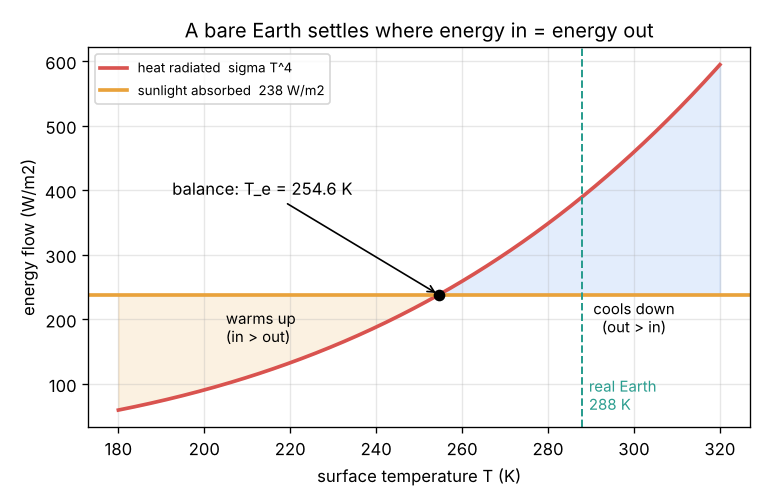
\includegraphics[width=0.85\linewidth]{figures/s01_energy_balance.png}\\\small Absorbed sunlight against heat radiated: they balance at 254.6 K, far below the real 288 K.\end{center}

\subsection*{E. Worked example}
For the Earth, S = 1361 W/m2 and alpha = 0.30. Find the absorbed sunlight, the bare-planet temperature, and how much the real 288 K surface radiates. How large is the greenhouse effect?
\begin{enumerate}[nosep]
\item Average sunlight per square metre: 1361 / 4 = 340.25 W/m2.
\item Absorbed: 340.25 x (1 - 0.30) = 238.2 W/m2.
\item Balance: T\_e\textasciicircum{}4 = 238.2 / (5.67 x 10\textasciicircum{}-8) = 4.20 x 10\textasciicircum{}9 K\textasciicircum{}4, so T\_e = fourth root = 254.6 K (-18.6 C).
\item The real surface at 288 K radiates 5.67 x 10\textasciicircum{}-8 x 288\textasciicircum{}4 = 390.1 W/m2, which is 152 W/m2 more than the planet absorbs from the Sun.
\item Greenhouse effect: 288 - 254.6 = 33.4 K.
\end{enumerate}
\textbf{Answer.} Absorbed 238.2 W/m2; bare Earth 254.6 K (-18.6 C); the real surface radiates 390.1 W/m2; the greenhouse effect is about 33 K.

\subsection*{F. Questions}
\begin{enumerate}[nosep]
\item \textbf{Conceptual.} Why do we divide the solar constant by 4, and not by 2 (only half the Earth is lit at a time)?
\item \textbf{Numerical.} Mars receives S = 586 W/m2 and has albedo 0.25. Find the absorbed sunlight and the bare-planet temperature. Check against the measured mean of about 210 K.
\item \textbf{Graph and simulation interpretation.} In the balance graph, the planet is at 230 K. Is it warming or cooling, and why? What happens to the gap between the two lines as it moves?
\item \textbf{Design and optimisation challenge.} Design: a bare Earth (S = 1361 W/m2) should have an equilibrium temperature of at least 273 K so that water does not freeze. What albedo is needed? Is that realistic? And what albedo makes a "snowball Earth" at 221 K?
\end{enumerate}

\section{Session 2: The one-layer greenhouse model}

\subsection*{A. Real-world problem}
Session 1 found that a bare Earth would sit at about 255 K (-18 C), but the real surface averages about 288 K (15 C). Nitrogen and oxygen let both sunlight and infrared pass, but water vapour and carbon dioxide (CO2), although only a small part of the air, absorb much of the infrared that the warm ground sends up. How much of that infrared must the air absorb to explain the missing 33 K, and what happens to the surface temperature if a little more is absorbed? (Simplified model of a global average; not a climate prediction.)

\subsection*{B. Concept and theory}
Put one thin layer of air above the surface. It is transparent to sunlight but absorbs a share epsilon of the infrared from the ground; the rest, (1 - epsilon), escapes through the "window". By Kirchhoff's law a layer that absorbs a share epsilon also emits epsilon sigma Ta\textasciicircum{}4 from each face, one up to space and one down to the ground. Three balances hold in equilibrium. Layer: it absorbs epsilon sigma Ts\textasciicircum{}4 and emits 2 epsilon sigma Ta\textasciicircum{}4, so sigma Ta\textasciicircum{}4 = sigma Ts\textasciicircum{}4 / 2 and Ta = Ts / 2\textasciicircum{}(1/4) whatever epsilon is. Top of the atmosphere: sunlight absorbed = window + layer up = (1 - epsilon / 2) sigma Ts\textasciicircum{}4. Surface: sunlight + back-radiation = sigma Ts\textasciicircum{}4, which then holds automatically. Solving gives Ts = Te [2 / (2 - epsilon)]\textasciicircum{}(1/4). With epsilon = 0 we get back Session 1; with epsilon = 1 the surface is 2\textasciicircum{}(1/4) = 1.19 times warmer, 302.7 K. Today's 288 K needs epsilon = 0.78. The key idea: the surface receives the back-radiation from the air as well as the sunlight, so it must get warmer to radiate it all away. With N layers that each absorb all infrared, Ts = Te (N + 1)\textasciicircum{}(1/4). A small rise in epsilon (more CO2) first cuts the outgoing infrared by sigma Ts\textasciicircum{}4 d(epsilon) / 2 before anything warms; this deficit is the radiative forcing.

\begin{itemize}[nosep]
\item epsilon: infrared absorptivity (= emissivity) of the layer (no unit)
\item Ts, Ta: surface and layer temperature (K)
\item Te: bare-planet temperature from Session 1 (254.6 K) (K)
\item OLR: outgoing longwave (infrared) radiation at the top (W/m2)
\item N: number of fully absorbing layers (no unit)
\item F: radiative forcing: drop in OLR when epsilon rises (W/m2)
\end{itemize}

\begin{equation*}
\text{layer:}\quad \varepsilon\,\sigma T_s^4 = 2\,\varepsilon\,\sigma T_a^4 \;\Rightarrow\; T_a = T_s/2^{1/4}
\end{equation*}

\begin{equation*}
\text{top:}\quad \frac{S(1-\alpha)}{4} = (1-\varepsilon)\,\sigma T_s^4 + \varepsilon\,\sigma T_a^4 = \left(1-\frac{\varepsilon}{2}\right)\sigma T_s^4
\end{equation*}

\begin{equation*}
T_s = T_e\left(\frac{2}{2-\varepsilon}\right)^{1/4} \qquad \varepsilon = 2\left[1-\left(\frac{T_e}{T_s}\right)^4\right]
\end{equation*}

\begin{equation*}
T_s = T_e\,(N+1)^{1/4}\ \text{(N opaque layers)} \qquad F = \tfrac12\,\sigma T_s^4\,\Delta\varepsilon
\end{equation*}

\begin{center}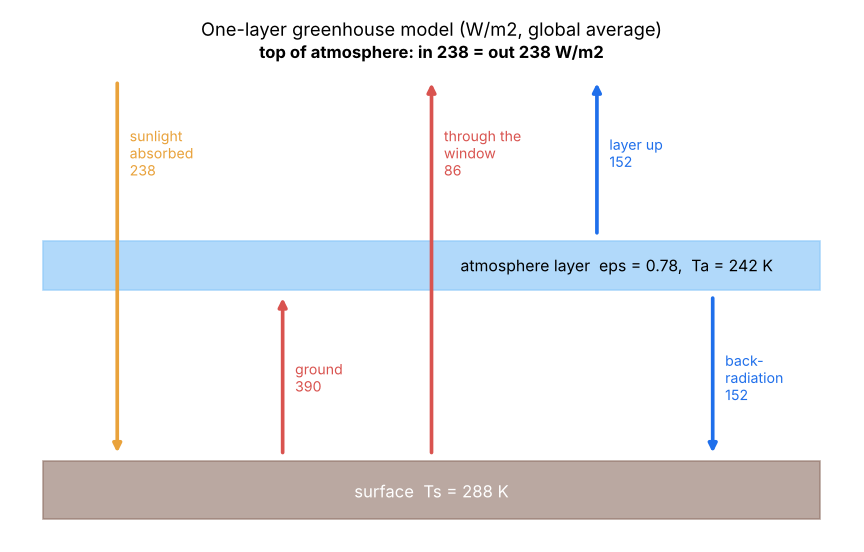
\includegraphics[width=0.85\linewidth]{figures/s02_layer_fluxes.png}\\\small Energy flows of the one-layer model for today's Earth, in W/m2.\end{center}

\subsection*{E. Worked example}
For the Earth (S = 1361 W/m2, alpha = 0.30) find the epsilon that gives a 288 K surface, the layer temperature, and every energy flow. Check all three balances.
\begin{enumerate}[nosep]
\item From Session 1, Te = 254.6 K. (Te / Ts)\textasciicircum{}4 = (254.6 / 288)\textasciicircum{}4 = 0.6105.
\item epsilon = 2 (1 - 0.6105) = 0.779.
\item Ta = 288 / 2\textasciicircum{}(1/4) = 288 / 1.1892 = 242.2 K.
\item Ground: sigma 288\textasciicircum{}4 = 390.1 W/m2. Window: (1 - 0.779) x 390.1 = 86.2 W/m2. Layer emission per face: 0.779 x sigma 242.2\textasciicircum{}4 = 0.779 x 195.1 = 151.9 W/m2.
\item Top: 86.2 + 151.9 = 238.1, about 238.2 W/m2 absorbed (rounding). Layer: absorbs 0.779 x 390.1 = 303.9 = 151.9 + 151.9 emitted. Surface: 238.2 + 151.9 = 390.1 = ground emission.
\end{enumerate}
\textbf{Answer.} epsilon = 0.779, Ta = 242.2 K; flows: ground 390.1, window 86.2, layer up 151.9, back-radiation 151.9 W/m2; all three balances close.

\subsection*{F. Questions}
\begin{enumerate}[nosep]
\item \textbf{Conceptual.} The layer emits only 152 W/m2 down, yet the surface is 33 K warmer than with no layer. Where does the extra warmth come from, if the Sun's input is unchanged?
\item \textbf{Numerical.} Find Ts and Ta for epsilon = 0.5 (S = 1361 W/m2, alpha = 0.30). Then find the epsilon needed for Ts = 290 K.
\item \textbf{Graph and simulation interpretation.} In the temperature graph, how much warmer can the surface get if epsilon goes from today's 0.78 all the way to 1? Why can one layer never give more?
\item \textbf{Design and optimisation challenge.} Design: the planet Venus receives S = 2601 W/m2, reflects 77 percent and has a surface at about 737 K. How many opaque layers does the N-layer model need? Then: for the Earth with N = 1, what must epsilon be for 288 K if clouds raise the albedo to 0.35?
\end{enumerate}

\section{Session 3: Simulate the warming and validate it}

\subsection*{A. Real-world problem}
Session 2 says that more infrared-absorbing gas means a warmer surface in equilibrium. But the ocean stores an enormous amount of heat, so the Earth cannot jump to its new temperature at once. If CO2 rises, how fast does the surface warm? How much warming is still to come after the CO2 stops rising? And what CO2 level would keep the long-term warming below 2 K? We build a step-by-step simulation, check it against exact answers, and then use it. (A simplified teaching model, not a climate projection.)

\subsection*{B. Concept and theory}
The top layer of the ocean (about 70 m, mixed by wind and waves) has a heat capacity C = rho c\_p h: 1025 kg/m3 x 3990 J/(kg K) x 70 m = 2.86 x 10\textasciicircum{}8 J/(m2 K), or 9.07 W yr/(m2 K) when divided by the seconds in a year. Any imbalance between absorbed sunlight and outgoing infrared warms it: C dTs/dt = S (1 - alpha) / 4 - (1 - epsilon / 2) sigma Ts\textasciicircum{}4. We step this forward with forward Euler, T\_new = T + dt x (in - out) / C. Near equilibrium we write T for the warming above the starting state: C dT/dt = F - lambda T. The forcing of CO2 grows with the logarithm of its concentration, F = 5.35 ln(CO2 / 280) W/m2 (Myhre et al. 1998), giving F2x = 3.71 W/m2 for doubled CO2. The feedback parameter lambda says how many extra W/m2 a 1 K warmer planet sheds. A planet that only radiates more (the Planck response) has lambda = 4 OLR / Ts = 3.3 W/(m2 K); water vapour, melting ice and clouds weaken this, and the IPCC's best estimate of the equilibrium climate sensitivity ECS = F2x / lambda is about 3 K (likely range 2.5 to 4 K), so lambda is about 1.24. For a sudden constant forcing the exact answer is T = (F / lambda)(1 - exp(-t / tau)) with time constant tau = C / lambda, which we use to test the code. While T is below F / lambda the planet still takes in N = F - lambda T: that heat goes into the ocean, and the warming it will still cause is "in the pipeline".

\begin{itemize}[nosep]
\item C: heat capacity of the ocean mixed layer per square metre (W yr/(m2 K))
\item T: warming above the starting equilibrium (K)
\item F: radiative forcing (F2x for doubled CO2) (W/m2)
\item lambda: feedback parameter: extra outgoing energy per kelvin of warming (W/(m2 K))
\item ECS: equilibrium climate sensitivity, F2x / lambda (K)
\item tau: time constant C / lambda (yr)
\item N: energy imbalance F - lambda T, heat going into the ocean (W/m2)
\item dt: time step of the simulation (yr)
\end{itemize}

\begin{equation*}
C\,\frac{dT_s}{dt} = \frac{S(1-\alpha)}{4} - \left(1-\frac{\varepsilon}{2}\right)\sigma T_s^4
\end{equation*}

\begin{equation*}
C\,\frac{dT}{dt} = F(t) - \lambda\,T,\qquad F = 5.35\,\ln\frac{\mathrm{CO_2}}{280}
\end{equation*}

\begin{equation*}
T_{\mathrm{eq}} = \frac{F}{\lambda},\qquad \mathrm{ECS} = \frac{F_{2\times}}{\lambda},\qquad \tau = \frac{C}{\lambda}
\end{equation*}

\begin{equation*}
T(t) = \frac{F}{\lambda}\left(1 - e^{-t/\tau}\right)\ \text{(step forcing)},\qquad T_{n+1} = T_n + \frac{\Delta t}{C}\,(F_n - \lambda T_n)
\end{equation*}

\begin{center}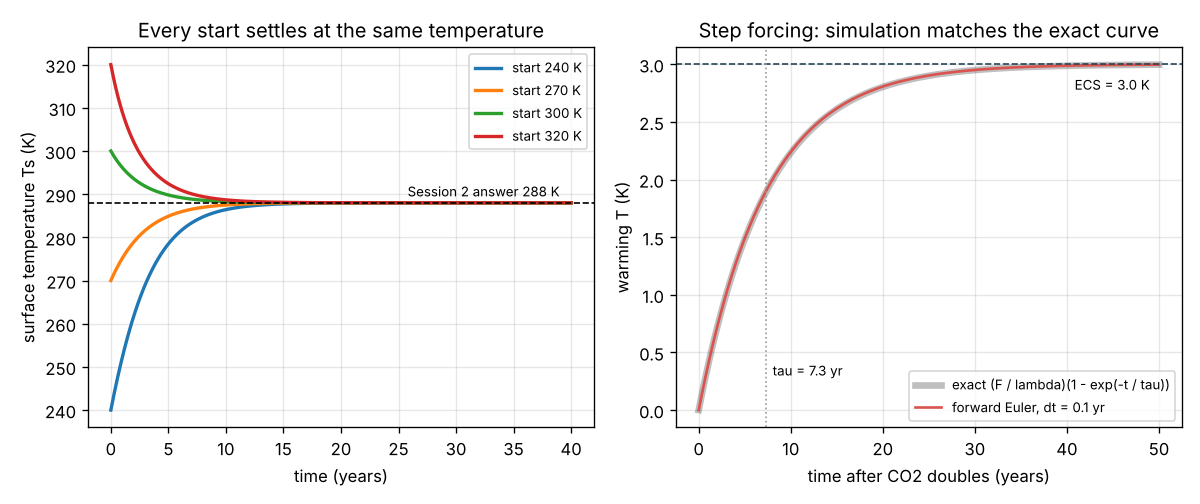
\includegraphics[width=0.85\linewidth]{figures/s03_validation.png}\\\small Left: the one-layer model relaxes to 288 K from any start. Right: Euler simulation against the exact step response.\end{center}

\subsection*{E. Worked example}
A 70 m ocean layer, ECS = 3 K. CO2 doubles overnight and then stays. Find C, lambda, tau, the warming after 10 years and the final warming; check the simulation and the energy balance.
\begin{enumerate}[nosep]
\item C = 1025 x 3990 x 70 / 3.156 x 10\textasciicircum{}7 = 9.07 W yr/(m2 K).
\item F2x = 5.35 x ln 2 = 3.708 W/m2; lambda = 3.708 / 3 = 1.236 W/(m2 K).
\item tau = C / lambda = 9.07 / 1.236 = 7.34 years.
\item After 10 years: T = 3 x (1 - exp(-10 / 7.34)) = 3 x (1 - 0.256) = 2.23 K. The Euler simulation with dt = 0.1 yr gives 2.24 K (error 0.007 K; it halves when dt halves).
\item Final warming F / lambda = 3.00 K. Energy check: heat stored C x T equals the sum of the imbalance N x dt over the run (27.185 W yr/m2 at 50 years, to round-off).
\end{enumerate}
\textbf{Answer.} C = 9.07 W yr/(m2 K), lambda = 1.236 W/(m2 K), tau = 7.3 yr; 2.23 K after 10 years, 3.00 K in the end; simulation and energy balance agree.

\subsection*{F. Questions}
\begin{enumerate}[nosep]
\item \textbf{Conceptual.} When CO2 stops rising, why does the Earth keep warming for a while? Use the energy imbalance N in your answer.
\item \textbf{Numerical.} With a 100 m ocean layer and ECS = 3 K, find C and tau. What share of the final warming is reached after one tau?
\item \textbf{Graph and simulation interpretation.} In the scenario figure, why does the ECS 4.5 K curve take longer to settle after year 70 than the Planck-only curve? Read the approximate times.
\item \textbf{Design and optimisation challenge.} Design: choose a CO2 ceiling (ppm) so that the equilibrium warming stays at or below 2 K for ECS = 2.5, 3 and 4 K. Which ceiling is safe for all three? Compare with about 420 ppm today.
\end{enumerate}

\section{Real-world mini-project}
\textbf{A CO2 ceiling for a 2 K limit.} A policy team asks: if the world wants long-term warming from CO2 of no more than 2 K above pre-industrial, what is the highest CO2 concentration it can stabilise at? Use \texttt{max\_co2\_for\_limit}, \texttt{lambda\_for\_ecs} and \texttt{run\_linear\_model} from Session 3 (70 m ocean, CO2 growing 1 percent a year from 280 ppm up to the ceiling, then held). Because the climate sensitivity is uncertain, answer for ECS = 2.5, 3 and 4 K. These numbers are for teaching; real budgets also count other gases, aerosols and the slow deep ocean.

\section{The path ahead}
\begin{enumerate}[nosep]
\item \textbf{Session 4: A two-box ocean.} A second, deep ocean box (heat capacity about 100 W yr/(m2 K)) linked to the surface layer by an exchange coefficient gamma (about 0.7 W/(m2 K)), stepped forward together.
\item \textbf{Session 5: Feedbacks one by one.} A lambda made of named parts (IPCC AR6 central values) and an ice-albedo feedback in which the albedo falls as the planet warms.
\item \textbf{Session 6: Other gases and aerosols.} Forcing functions for CH4 and N2O and a simple aerosol forcing, added to the CO2 forcing.
\item \textbf{Session 7: The historical record, 1850 to today.} A loader for a published annual forcing series and a global temperature record (both free), and a run of the two-box model from 1850.
\item \textbf{Session 8: Carbon budgets and future paths.} A simple carbon cycle that turns emissions (GtC per year) into CO2 concentration, and three future emission paths.
\end{enumerate}

\section{Answers and hints}

\subsection*{Session 1}
\begin{enumerate}[nosep]
\item \textbf{Conceptual.} Hint: Compare the area that catches the sunlight with the area that radiates heat away. Solution: The Earth catches sunlight like a flat disc of area pi R\textasciicircum{}2 (its shadow). It radiates heat from its whole surface, a sphere of area 4 pi R\textasciicircum{}2, day and night. The ratio is pi R\textasciicircum{}2 / (4 pi R\textasciicircum{}2) = 1 / 4. Dividing by 2 would count the day side as if it faced the Sun straight on everywhere; in fact the sunlight is slanted near the edges, and that slant brings the day-side average down to S / 2 and the whole-sphere average to S / 4.
\item \textbf{Numerical.} Hint: Absorbed = S (1 - alpha) / 4, then take the fourth root of absorbed / sigma. Solution: Absorbed = 586 x 0.75 / 4 = 109.9 W/m2. T\textasciicircum{}4 = 109.9 / 5.67 x 10\textasciicircum{}-8 = 1.94 x 10\textasciicircum{}9 K\textasciicircum{}4, so T = 209.8 K. This is within 1 K of the measured 210 K: Mars has a very thin atmosphere, so its greenhouse effect is tiny and the bare model works well.
\item \textbf{Graph and simulation interpretation.} Hint: Read the absorbed line and the T\textasciicircum{}4 curve at 230 K. Solution: At 230 K the planet radiates 5.67 x 10\textasciicircum{}-8 x 230\textasciicircum{}4 = 158.7 W/m2 but absorbs 238.2 W/m2, so it gains 79.5 W/m2 and warms. As T rises the T\textasciicircum{}4 curve climbs toward the flat line and the gap shrinks to zero at 254.6 K, where the warming stops. From above (say 280 K) the gap is negative and the planet cools back to the same point: the balance is stable.
\item \textbf{Design and optimisation challenge.} Hint: Invert: 1 - alpha = 4 sigma T\textasciicircum{}4 / S. Solution: 1 - alpha = 4 x 5.67 x 10\textasciicircum{}-8 x 273\textasciicircum{}4 / 1361 = 0.926, so alpha must be at most 0.074, darker than the open ocean almost everywhere and with no clouds at all. That is not realistic: clouds alone reflect about 0.2. So a bare Earth would be frozen, and the warmth we enjoy needs the atmosphere. For alpha = 0.60 (mostly ice and snow) the model gives 221 K. Trade-off: a darker planet is warmer, but albedo alone cannot explain 288 K.
\end{enumerate}

\subsection*{Session 2}
\begin{enumerate}[nosep]
\item \textbf{Conceptual.} Hint: Write the surface balance with and without the layer. Solution: Without the layer the ground receives only 238 W/m2 and must radiate 238, so it sits at 255 K. With the layer it receives 238 from the Sun plus 152 back from the layer, 390 W/m2 in all, and must radiate 390, which needs 288 K. No energy is created: the layer recycles part of the ground's own infrared. At the top of the atmosphere the planet still sends 238 W/m2 to space, the same as it absorbs.
\item \textbf{Numerical.} Hint: Ts = 254.6 x (2 / (2 - eps))\textasciicircum{}(1/4); invert with eps = 2 (1 - (Te / Ts)\textasciicircum{}4). Solution: eps = 0.5: 2 / 1.5 = 1.333, fourth root 1.0746, so Ts = 254.6 x 1.0746 = 273.6 K and Ta = 273.6 / 1.1892 = 230.0 K. For 290 K: (254.6 / 290)\textasciicircum{}4 = 0.5939, so eps = 2 x 0.4061 = 0.812. Sanity check: 0.812 lies between 0.779 (288 K) and 1, as it must.
\item \textbf{Graph and simulation interpretation.} Hint: Read Ts at eps = 1 and compare with the N-layer panel. Solution: At eps = 1, Ts = 2\textasciicircum{}(1/4) x 254.6 = 302.7 K, only 14.7 K more than 288 K. A single layer that absorbs everything can at most send back half of what it absorbs, so the surface flux is at most twice the solar input and Ts at most 2\textasciicircum{}(1/4) Te. More warming needs more layers (or a thicker atmosphere): the N-layer panel shows 335 K for N = 2 and 381 K for N = 4.
\item \textbf{Design and optimisation challenge.} Hint: N = (Ts / Te)\textasciicircum{}4 - 1, with Te from Session 1 for Venus. Solution: Venus: absorbed = 2601 x 0.23 / 4 = 149.6 W/m2, Te = 226.6 K. (737 / 226.6)\textasciicircum{}4 = 111.9, so N = about 111 layers: a very thick, infrared-opaque atmosphere. Earth with alpha = 0.35: Te = 249.9 K, (249.9 / 288)\textasciicircum{}4 = 0.567, eps = 2 x 0.433 = 0.87. Trade-off: a brighter, cloudier Earth absorbs less sunlight, so it needs a stronger greenhouse to stay at 288 K. The real atmosphere is not a stack of layers, but the count shows how opaque Venus's air is.
\end{enumerate}

\subsection*{Session 3}
\begin{enumerate}[nosep]
\item \textbf{Conceptual.} Hint: What is N = F - lambda T on the day the CO2 stops rising? Solution: On that day F is at its final value but T is still below F / lambda, because the ocean needs time to heat up. So N = F - lambda T is still positive: the planet absorbs more than it sends out. That extra energy keeps warming the ocean until lambda T = F and N = 0. In the 3 K case the warming at year 70 is 2.68 K, so about 0.3 K more is "in the pipeline". In the real world the deep ocean makes this tail last centuries.
\item \textbf{Numerical.} Hint: C scales with depth; at t = tau the factor is 1 - exp(-1). Solution: C = 1025 x 3990 x 100 / 3.156 x 10\textasciicircum{}7 = 12.96 W yr/(m2 K). tau = 12.96 / 1.236 = 10.5 years. After one tau the warming is 1 - exp(-1) = 0.632 of its final value, 63 percent (1.90 K of 3 K). A deeper layer warms more slowly but to the same final temperature.
\item \textbf{Graph and simulation interpretation.} Hint: tau = C / lambda: which case has the smaller lambda? Solution: tau = 9.07 / 3.31 = 2.7 yr for Planck only, but 9.07 / 0.82 = 11 yr for ECS 4.5 K. A small lambda means the planet sheds little extra heat per kelvin, so the imbalance closes slowly. In the figure the Planck curve settles a few years after year 70; the 4.5 K curve takes about 40 to 50 years (several tau). A more sensitive climate warms more and also takes longer to show it.
\item \textbf{Design and optimisation challenge.} Hint: CO2\_max = 280 exp(2 lambda / 5.35) with lambda = 3.708 / ECS. Solution: ECS 2.5 K: lambda = 1.483, CO2\_max = 280 exp(0.554) = 488 ppm. ECS 3 K: lambda = 1.236, 280 exp(0.462) = 444 ppm. ECS 4 K: lambda = 0.927, 280 exp(0.347) = 396 ppm. Only 396 ppm is safe for all three, and today's level is already above it. Trade-off: planning for the central estimate (444 ppm) leaves a real chance of exceeding 2 K; the model also ignores other gases, which add forcing, and aerosols, which remove some.
\end{enumerate}

\section{How to join}
Read \texttt{CONTRIBUTING.md} in the repository, then pick an issue labelled \texttt{good first issue}. Repository: \url{https://github.com/KrunalPanchal1995/pan-iit-oss/tree/main/openclimate}

\end{document}
